\section{Experimental Results}
\label{sec:results}

\subsection{Experimental Platform}
\label{sec:summit}

All the experiments in this section were conducted on Summit. Summit is a supercomputer created by IBM for the Oak Ridge National Laboratory. 
There are approximately 4,600 nodes on Summit. Each node contains two IBM POWER9 processors on separate sockets with dual NVLINK bricks to facilitate a transfer rate of 
25 GB/s between the processors. Each node contains 512 GB of DDR4 memory for use by both processors. Each POWER9 processor utilizes 22 IBM SIMD Multi-Cores (SMCs), 
although one of these SMCs on each processor is dedicated to memory transfer and is therefore not available for computation. 
For node scaling experiments, all 42 available SMCs were utilized in each node so that every node computed with 42 separate MPI processes.
Additionally, every node also supports six NVIDIA Volta V100 accelerators but these were unused by our algorithm. 

H2NMF uses the Armadillo library (version 9.900.1) for all matrix operations. 
In Armadillo, sparse matrices are stored in Compressed Sparse Column (CSC) format and dense matrices are stored in column-major ordering.
On Summit, we linked this version of Armadillo with OpenBLAS (version 0.3.9) and IBM's Spectrum MPI (version 10.3.1.2-20200121).


\GB{specify that $\imath=\jmath=100$ in all experiments, also what do we set $k$ to be?  fixed number for each dataset?  any other experimental parameters we should specify? could also specify these at the beginning of \Cref{sec:perf}}


\subsection{Datasets}
\begin{itemize}
	\item \textit{Hyperspectral Imaging}:
	For Hyperspectral imaging, we chose the Hyperspectral digital imagery collection experiment (HYDICE) image of the Washington DC Mall. We will refer
	to this dataset as \hyper{}\cite{DC-HYDICE}.
	
	\hyper{} is formatted into a 3-way tensor representing two spatial dimensions of pixels and one dimension of spectral bands. So, a slice along
	the spectral band dimnesion would be the full \hyper{} image in that spectral band. For H2NMF, these tensors are flattened so that the rows represent the
	$191$ spectral bands and the columns represent the $392960$ pixels. 

	Larger hyperspectral datasets tend to not grow larger than around 200 spectral bands and have millions or billions of pixels. So, scaling is 
	limited for this dataset given our data distribution scheme.
	\item \textit{Image Classification}:
	Image Classification datasets contain tens of thousands of images of equal size. The dataset we chose is the SIIM-ISIC Melanoma classification
	dataset, which we will refer to as \image{}\cite{SIIM-ISIC}. \image{} consists of $33126$ RGB training images equally sized at $1024 \times 1024$. Unlike with hyperspectral imaging, the resulting
	matrix used in H2NMF consists of image pixels along the rows and individual images along the columns. So, the resulting sized matrix is
	$3145728 \times 33126$, which is approximately 800GB in size. 

	Given its size, \image{} can only scale from $10$ Summit nodes.
	\item \textit{Synthetic Dataset}:
	Our synthetic dataset is the same shape of \image{} but consists of fewer rows and columns by a factor of $3$. The resulting matrix is $1048576 \times 11042$. 
	We chose a smaller size dataset to better see the limits of scaling and to scale from fewer Summit nodes.
\end{itemize}

\subsection{Performance}
\label{sec:perf}

\subsubsection{Single-Node Scaling for DC Dataset}

\GB{add only speedup plot for entire tree (at least all complete levels) from 1 core to 42 cores}

\begin{itemize}
	\item emphasize we start with a small data set that fits on one node and has only 191 rows
	\item using 1 node (2 sockets), because we are memory bandwidth bound we expect limited speedup but we can save time with parallelism even for this small a data set
\end{itemize}

\subsubsection{Rank-2 NMF Strong Scaling}

We perform strong scaling experiments for a single Rank-2 NMF (\Cref{alg:parrank2nmf}) on the synthetic and \image{} datasets.
The theory (\Cref{eq:r2nmfcost}) suggests that perfect strong scaling is possible as long as the execution time is dominated by local computation.
Both the matrix multiplications and NNLS solves scale linearly with $1/p$ (we expect MatMul to dominate), but the bandwidth cost is independent of $p$ and the latency cost increases slightly with $p$.

\Cref{fig:synrank2speedup,fig:rwrank2speedup} show performance relative to the smallest number of nodes required to store data and factor matrices.
The synthetic data is chosen to fit on a single node, while the \image{} data requires 10 nodes to store the input matrix as well as temporary and output matrices.
For these data sets, we observe nearly perfect strong scaling, with 47$\times$ speedup on 50 nodes (over 1 node) for synthetic data and 7.1$\times$ speedup on 80 nodes (over 10 nodes) for \image{} data.

\begin{figure}
\begin{center}
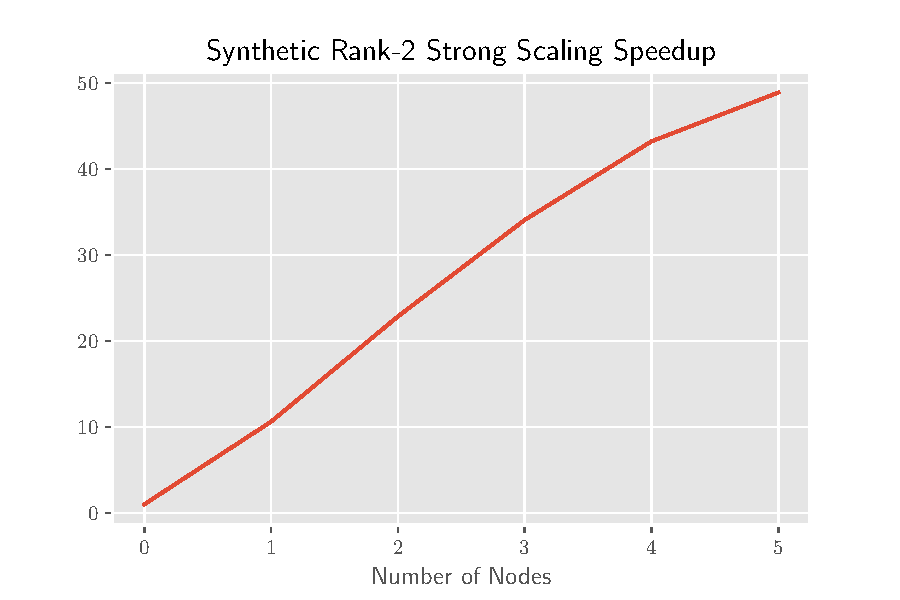
\includegraphics[height=2in, width=\columnwidth]{plots/synthetic_rank2_speedup.pdf}
\caption{Strong Scaling Speedup for Rank-2 NMF on synthetic data}
\label{fig:synrank2speedup}
\end{center}
\end{figure}

\begin{figure}
\begin{center}
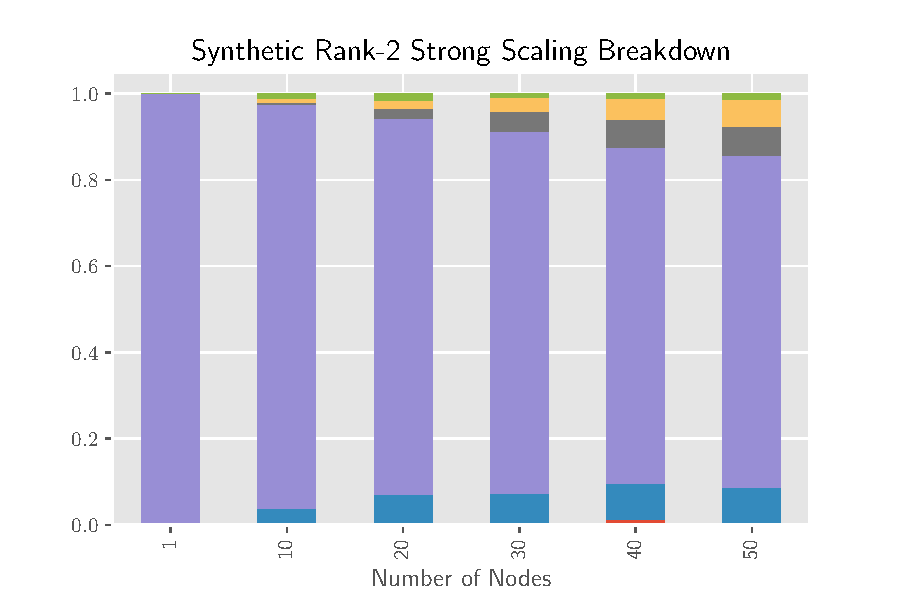
\includegraphics[height=2in, width=\columnwidth]{plots/synthetic_rank2_strongscaling.pdf}
\caption{Relative Time Breakdown for Rank-2 NMF on synthetic data}
\label{fig:synrank2strongscaling}
\end{center}
\end{figure}

The relative time breakdowns are presented in \Cref{fig:synrank2strongscaling,fig:rwrank2strongscaling} and explain the strong scaling performance.
Each experiment is normalized to 100\% time, so comparisons cannot be readily made across numbers of compute nodes. 
For both data sets, we see that the time is dominated by MatMul, which is the primary reason for the scalability.
The dominant matrix multiplications are between a large matrix and a matrix with 2 columns, so it is locally memory bandwidth bound, with performance proportional to the size of the large matrix.
In each plot, we also see the relative time of all-gather and reduce-scatter increasing, which is because the local computation is decreasing while the communication cost is slightly increasing with $p$.
This pattern will continue as $p$ increases, which will eventually limit scalability, but for these data sets the MatMul takes around 80\% of the time at over 2000 cores.

\begin{figure}
\begin{center}
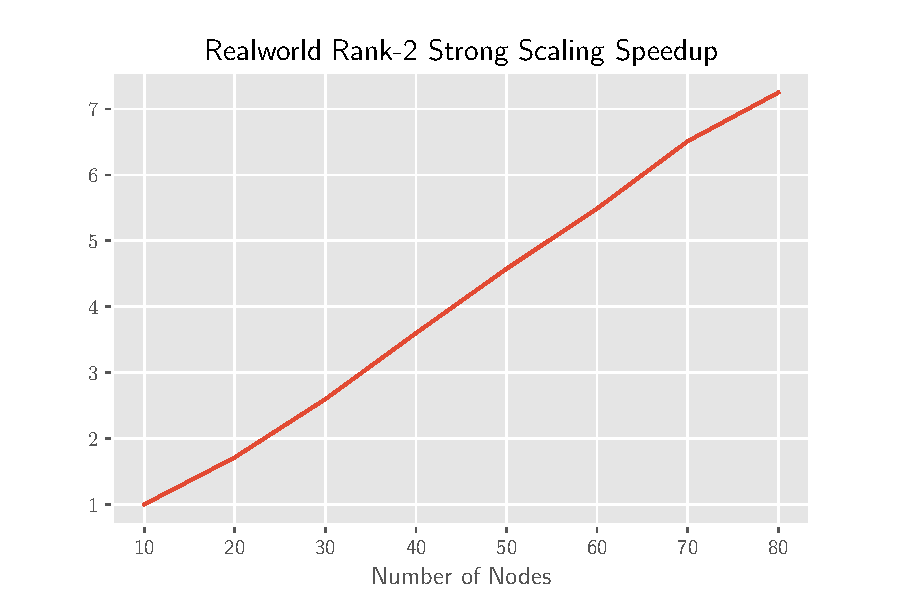
\includegraphics[height=2in, width=\columnwidth]{plots/realworld_rank2_speedup.pdf}
\caption{Strong Scaling Speedup for Rank-2 NMF on \image{} data}
\label{fig:rwrank2speedup}
\end{center}
\end{figure}

\begin{figure}
\begin{center}
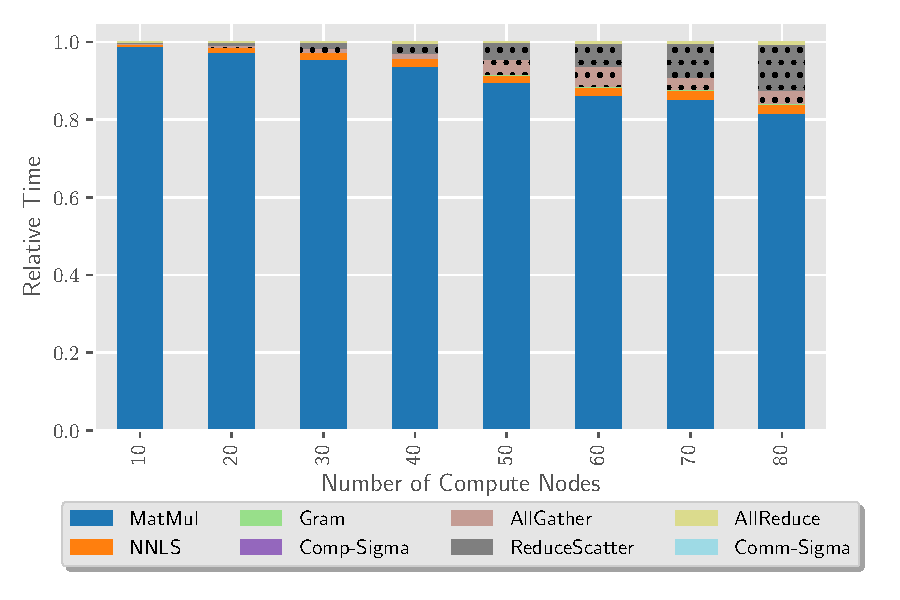
\includegraphics[height=2in, width=\columnwidth]{plots/realworld_rank2_strongscaling.pdf}
\caption{Relative Time Breakdown for Rank-2 NMF on \image{} data}
\label{fig:rwrank2strongscaling}
\end{center}
\end{figure}



\subsubsection{Hierarchical Clustering Strong Scaling}

\GB{Do these breakdowns include the score function?  actually this may explain why all-reduce costs more, it also has $O(n)$ data for score...}

\GB{4 plots: 2 data sets with speedup/breakdown, note that we include time for complete levels, ignoring nodes in incomplete levels for easier interpretation}

From equation \ref{eq:treecost}, we expect to see perfect strong scaling in a computationally bound H2NMF problem with fixed frontier node $k$ count.
However, the problem should become latency bound with its $\log p$ cost as we scale. Figure \ref{fig:fig:synhierspeedup} shows this latency limit as
we scale to 50 compute nodes on the synthetic data. Figure \ref{fig:synhierstrongscaling}

From equation \ref{eq:levelcost}
\begin{itemize}
	\item theory (\Cref{eq:treecost}) says...
	\item Fig 7 shows limit of strong scaling for synthetic data (time increases at 50 nodes compared to 40), Fig 8 gives breakdown and explains
	\begin{itemize}
		\item drastic performance dropoff may be artifact of all-gather, which should take about the same time as reduce-scatter, but speedup from 30 to 40 nodes is also slight
		\item by 50 nodes, about 50\% of time in communication; still mostly dominated by bandwidth cost because ag and rs dominate ar
		\item note the difference between the scaling of single rank-2 and entire tree: poor scaling must be due to lower levels, which we explore in the next section
	\end{itemize}
	\item Fig 9 shows reasonable scaling for entire tree -- speedup drops from 7x to 6x over 80 nodes; Fig 10 shows that MM is still 70\% of run time on 80 nodes, which allows for near-linear scaling
\end{itemize}

\begin{figure}
\begin{center}
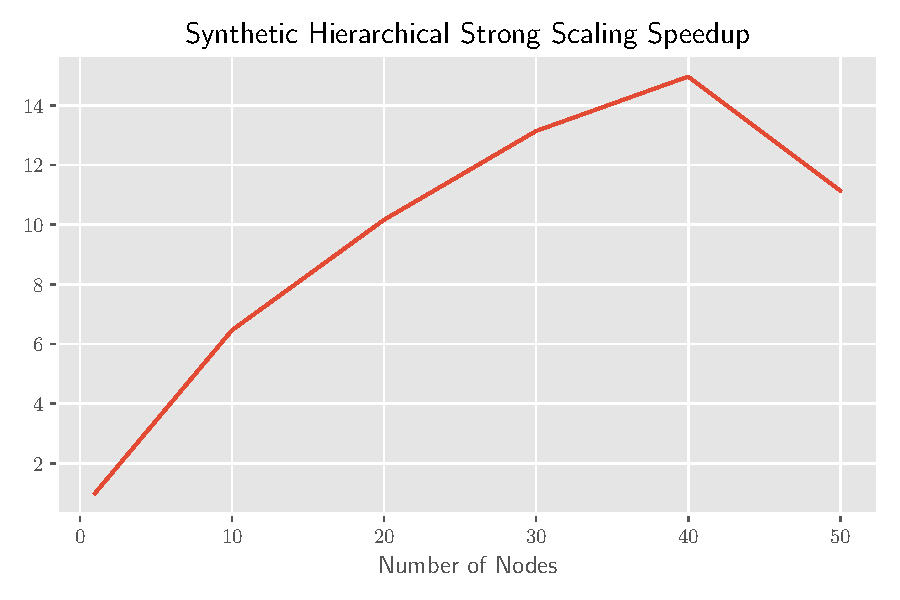
\includegraphics[height=2in, width=\columnwidth]{plots/synthetic_hierarchical_speedup.pdf}
\caption{Strong Scaling Speedup for Hierarchical Clustering. The total time taken for complete Hierarchical Clustering \cref{alg:hiernmf2}}
\label{fig:synhierspeedup}
\end{center}
\end{figure}

\begin{figure}
\begin{center}
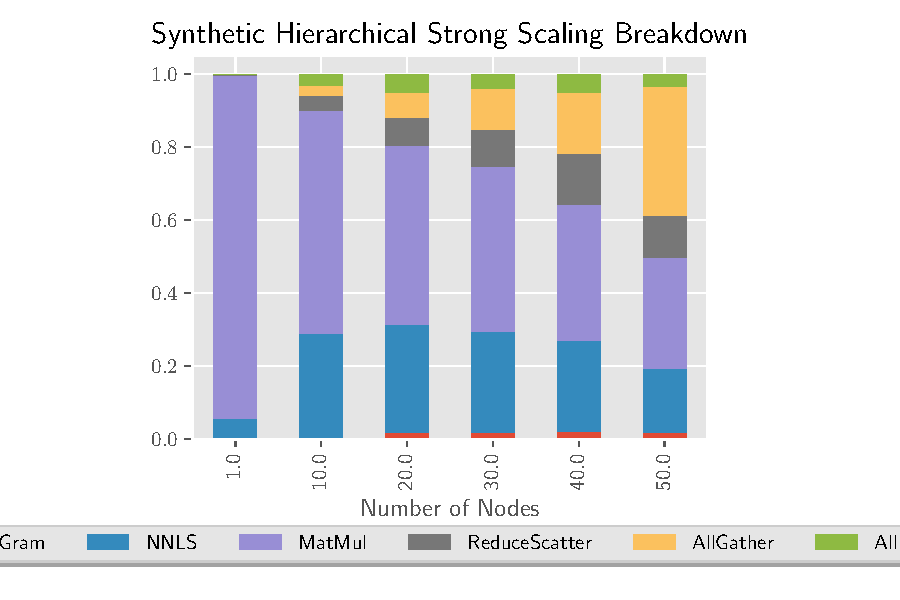
\includegraphics[height=2in, width=\columnwidth]{plots/synthetic_hier_strongscaling.pdf}
\caption{Relative Time Breakdown for Hierarchical Clustering. The plot uses the total time taken for complete Hierarchical Clustering \cref{alg:hiernmf2}}
\label{fig:synhierstrongscaling}
\end{center}
\end{figure}

\begin{figure}
\begin{center}
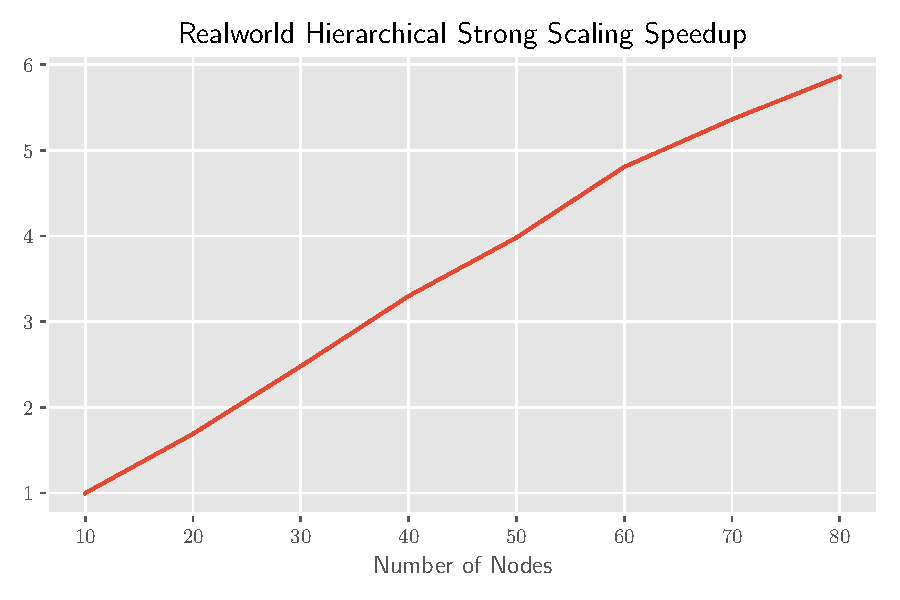
\includegraphics[height=2in, width=\columnwidth]{plots/realworld_hierarchical_speedup.pdf}
\caption{Strong Scaling Speedup for Hierarchical Clustering on \image{} Data. The total time taken for complete Hierarchical Clustering \cref{alg:hiernmf2}}
\label{fig:rwhierspeedup}
\end{center}
\end{figure}

\begin{figure}
\begin{center}
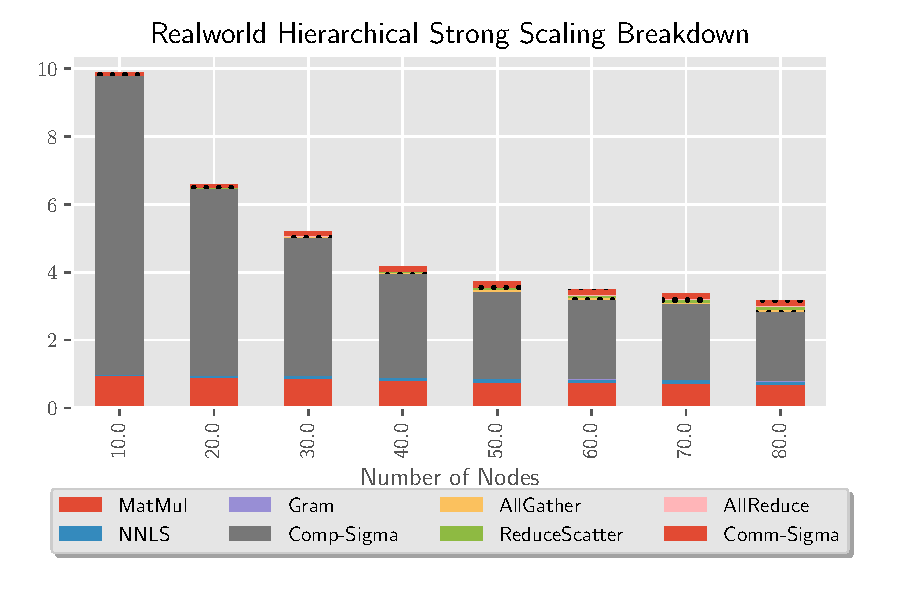
\includegraphics[height=2in, width=\columnwidth]{plots/realworld_hier_strongscaling.pdf}
\caption{Relative Time Breakdown for Hierarchical Clustering on \image{}. The plot uses the total time taken for complete Hierarchical Clustering \cref{alg:hiernmf2}}
\label{fig:rwhierstrongscaling}
\end{center}
\end{figure}

\subsubsection{Level Scaling}

\GB{3 plots: for synthetic level breakdown for 1 node and for 40 nodes; for realworld just for 80 nodes}

\begin{itemize}
	\item theory says per-level cost is \Cref{eq:levelcost}
\end{itemize}

\begin{figure}
\begin{center}
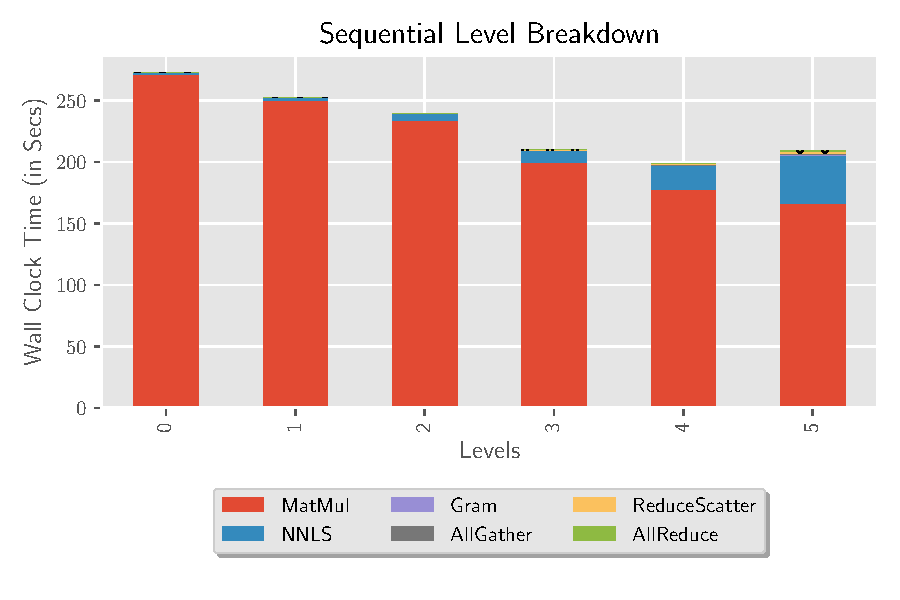
\includegraphics[height=2in, width=\columnwidth]{plots/synthetic_sequential_level_breakdown.pdf}
\caption{Sequential Breakdown plot for levels 0 to 5. y-axis is absolute wall clock time in seconds}
\label{fig:seqlevelbreakdown}
\end{center}
\end{figure}

\begin{figure}
\begin{center}
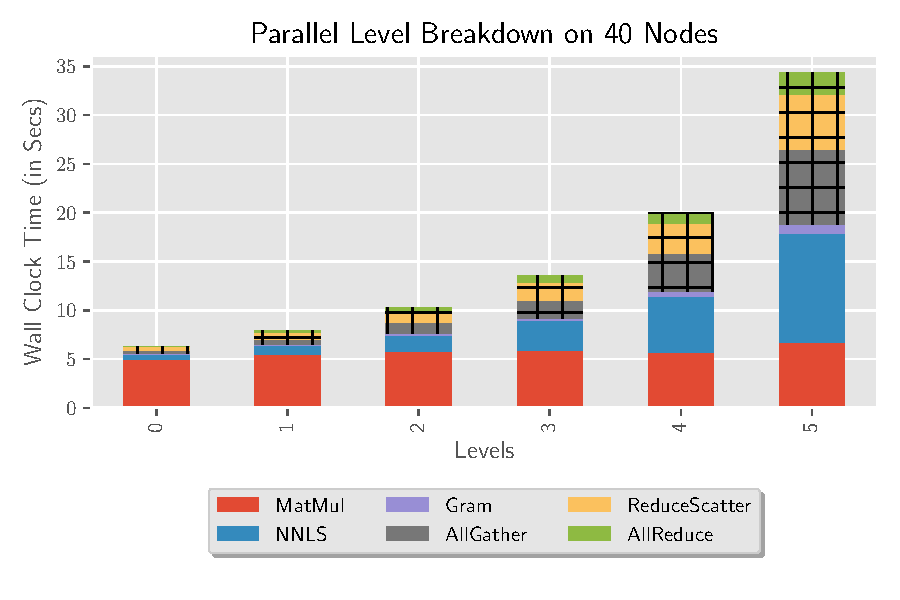
\includegraphics[height=2in, width=\columnwidth]{plots/synthetic_parallel_level_breakdown.pdf}
\caption{Parallel Breakdown plot for levels 0 to 5 on 40 nodes. y-axis is absolute wall clock time in seconds}
\label{fig:parallellevelbreakdown}
\end{center}
\end{figure}


\begin{figure}
\begin{center}
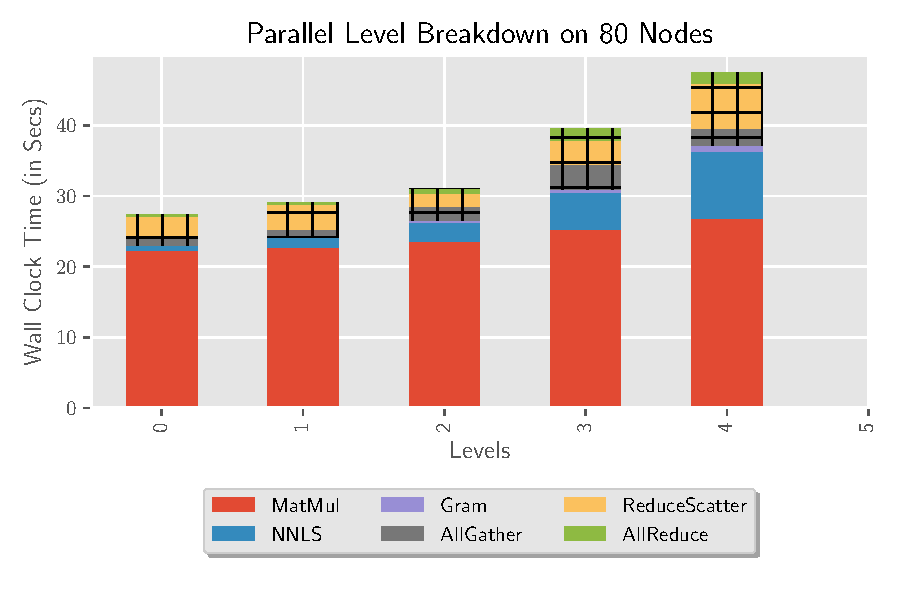
\includegraphics[height=2in, width=\columnwidth]{plots/realworld_parallel_level_breakdown.pdf}
\caption{Parallel Breakdown plot for levels 0 to 5 on 80 nodes. y-axis is absolute wall clock time in seconds}
\label{fig:rwparallellevelbreakdown}
\end{center}
\end{figure}


\subsection{DC Clustering Results}

\subsubsection{Hyperspectral Imaging}
\begin{figure}
% !TEX root = ../paper.tex

\resizebox{\columnwidth}{!}{
\begin{tikzpicture}
    \node[inner sep=0pt] (original) at (0,0)
        {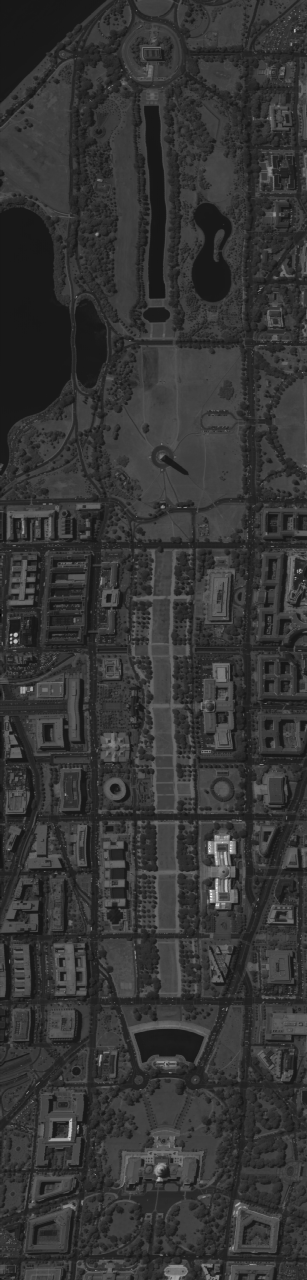
\includegraphics[width=0.8cm,height=3.2cm]{data/DC/0.png}};
        \draw[thick,->] (-0.4,0.8) .. controls (-3,0.8) .. (-3,-0.4);
        \node[inner sep=0pt] (1) at (-3,-2)
            {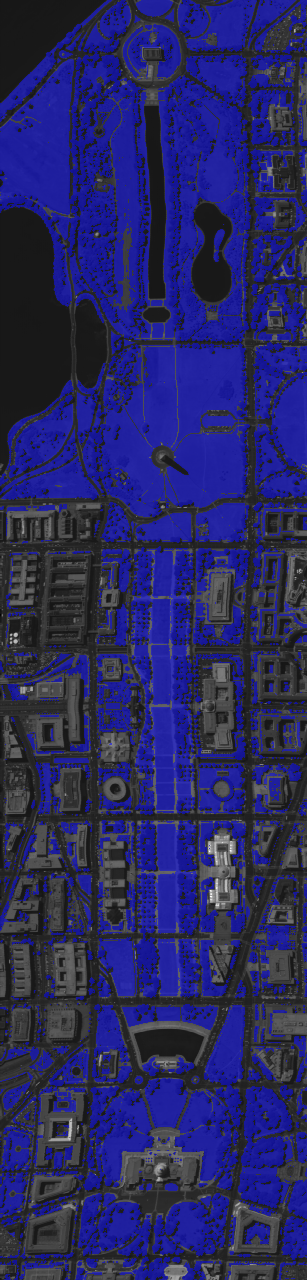
\includegraphics[width=0.8cm,height=3.2cm]{data/DC/1.png}};
            \draw[thick,->] (-2.6,-1.2) .. controls (-1.6,-1.2) .. (-1.6,-2.4);
            \node[inner sep=0pt] (3) at (-1.6,-4)
                {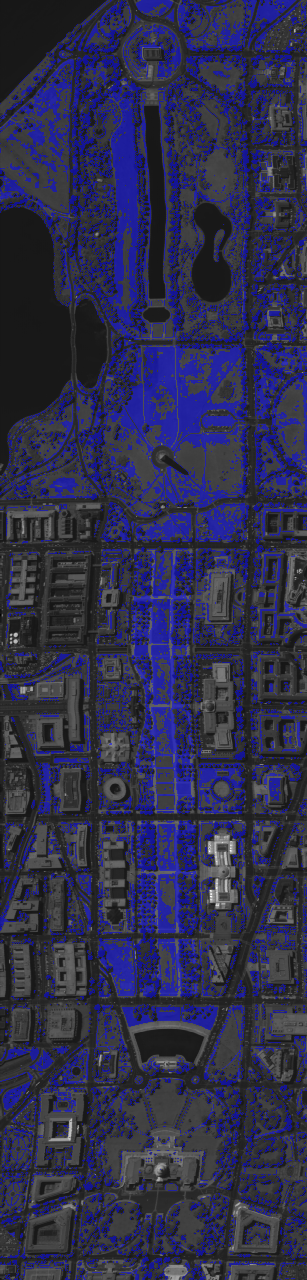
\includegraphics[width=0.8cm,height=3.2cm]{data/DC/3.png}};
                \draw[thick,->] (-2,-3.2) .. controls (-2.5,-3.2) .. (-2.5,-4.4);
                \node[inner sep=0pt] (7) at (-2.5,-6)
                    {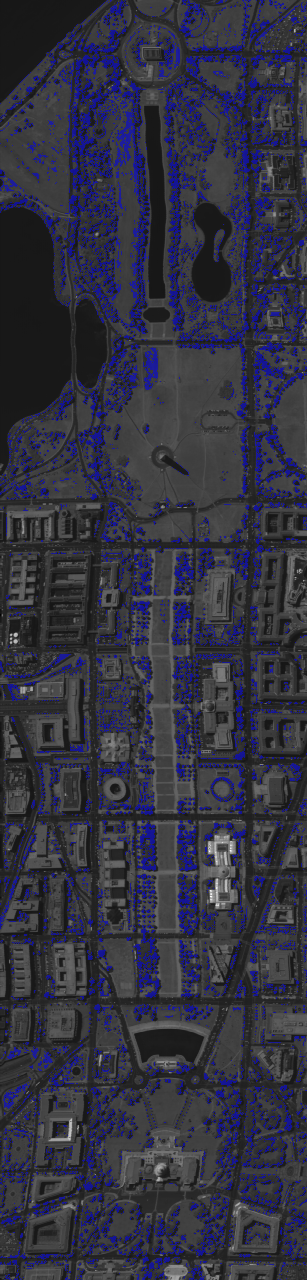
\includegraphics[width=0.8cm,height=3.2cm]{data/DC/7.png}};
                \draw[thick,->] (-1.2,-3.2) .. controls (-0.7,-3.2) .. (-0.7,-4.4);
                \node[inner sep=0pt] (8) at (-0.7,-6)
                    {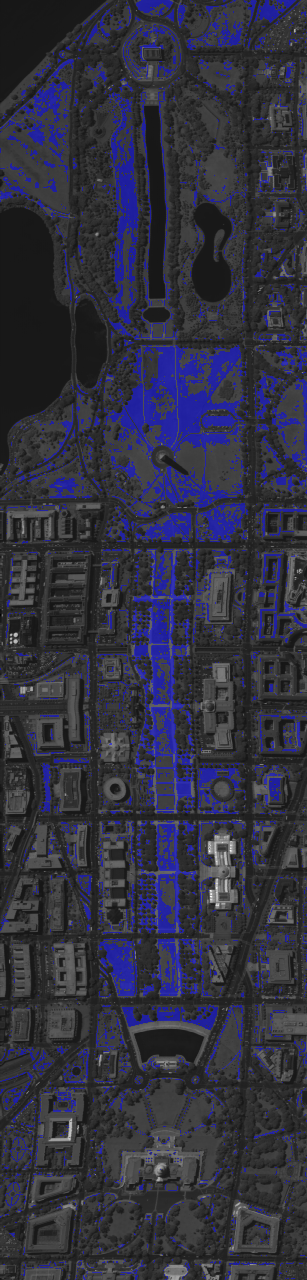
\includegraphics[width=0.8cm,height=3.2cm]{data/DC/8.png}};
            \draw[thick,->] (-3.4,-1.2) .. controls (-4.4,-1.2) .. (-4.4,-2.4);
            \node[inner sep=0pt] (4) at (-4.4,-4)
                {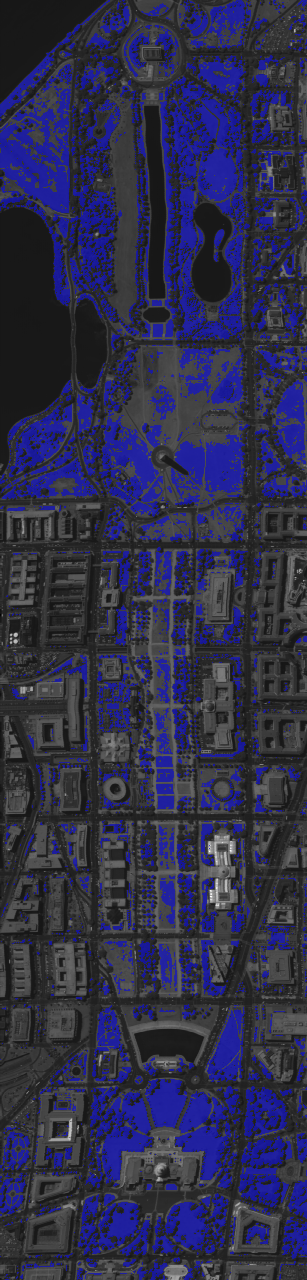
\includegraphics[width=0.8cm,height=3.2cm]{data/DC/4.png}};
        \draw[thick,->] (0.4,0.8) .. controls (3,0.8) .. (3,-0.4);
        \node[inner sep=0pt] (2) at (3,-2)
            {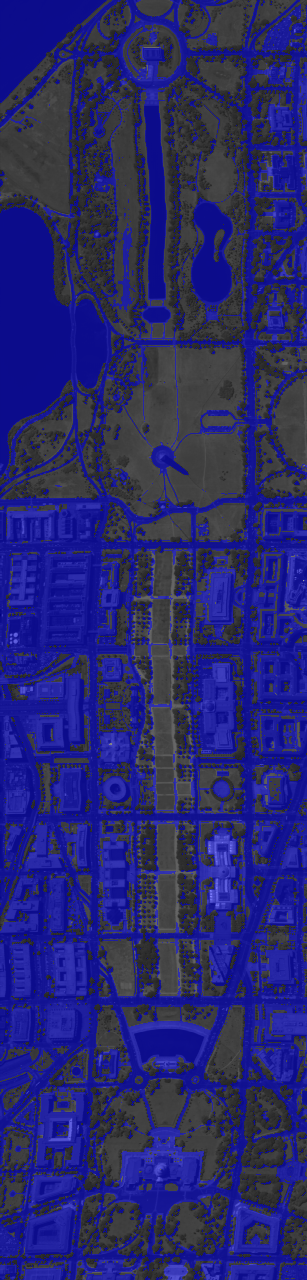
\includegraphics[width=0.8cm,height=3.2cm]{data/DC/2.png}};
            \draw[thick,->] (3.4,-1.2) .. controls (4.4,-1.2) .. (4.4,-2.4);
            \node[inner sep=0pt] (5) at (4.4,-4)
                {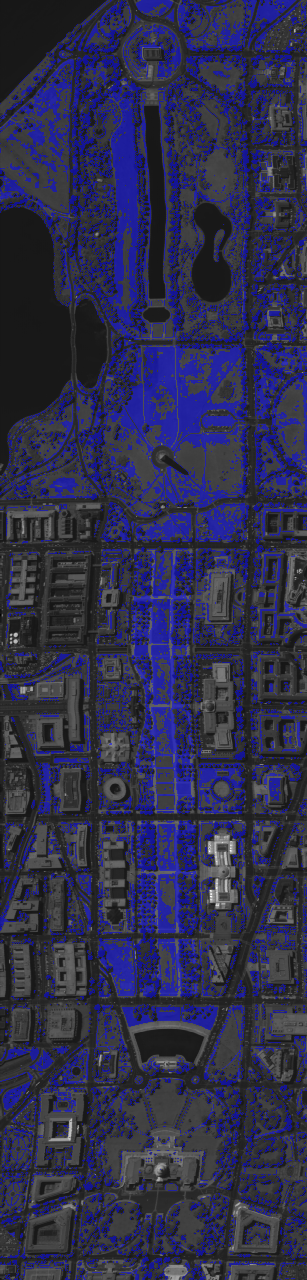
\includegraphics[width=0.8cm,height=3.2cm]{data/DC/3.png}};
            \draw[thick,->] (2.6,-1.2) .. controls (1.6,-1.2) .. (1.6,-2.4);
            \node[inner sep=0pt] (6) at (1.6,-4)
                {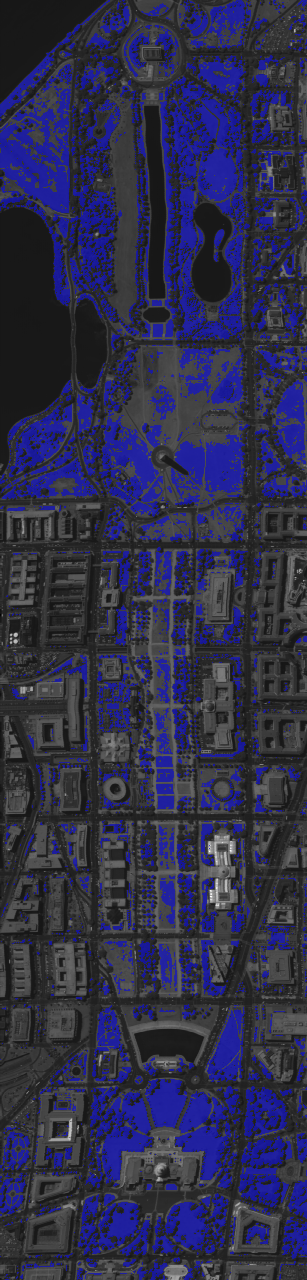
\includegraphics[width=0.8cm,height=3.2cm]{data/DC/4.png}};
                \draw[thick,->] (1.2,-3.2) .. controls (0.7,-3.2) .. (0.7,-4.4);
                \node[inner sep=0pt] (13) at (0.7,-6)
                    {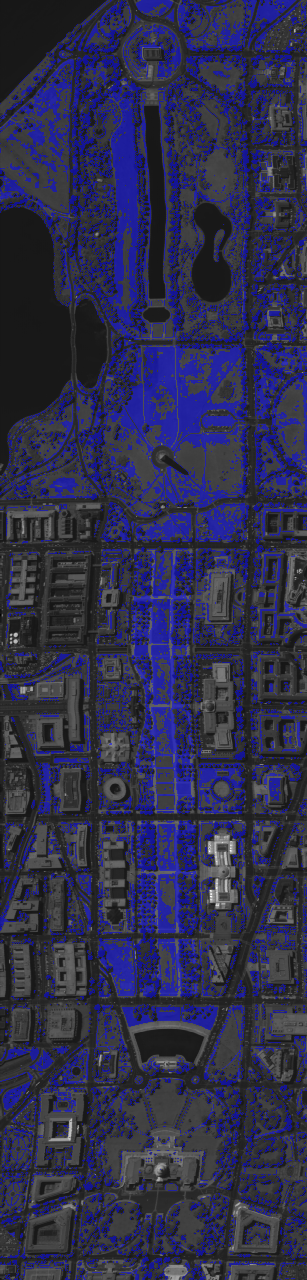
\includegraphics[width=0.8cm,height=3.2cm]{data/DC/3.png}};
                    \draw[thick,->] (2,-3.2) .. controls (2.5,-3.2) .. (2.5,-4.4);
                \node[inner sep=0pt] (14) at (2.5,-6)
                    {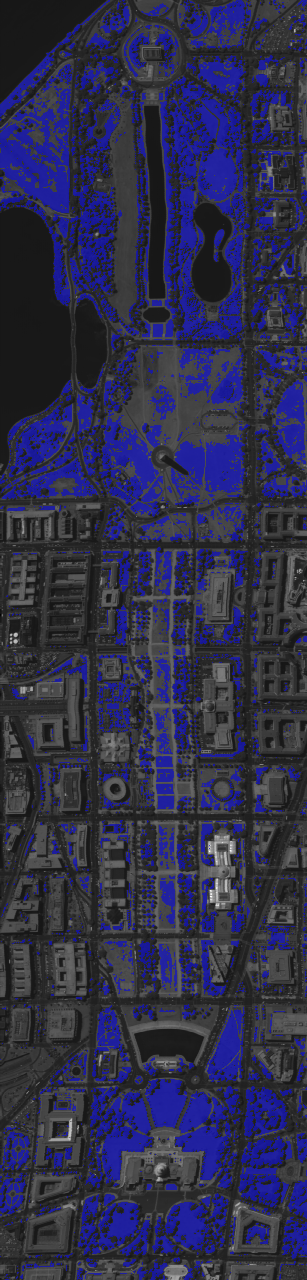
\includegraphics[width=0.8cm,height=3.2cm]{data/DC/4.png}};
\end{tikzpicture}
}
\caption{Hierarchical Cluster from DC Mall Image}
\label{fig:dc}
\end{figure}
